%  !TeX  root  =  user_guide.tex 

\section{Plugin GDALTools}\label{label_plugingdaltools}

% when the revision of a section has been finalized, 
% comment out the following line:
% \updatedisclaimer

\subsection{Cos'è GDALTools?}\label{whatsgdal}
Il plugin GDALTools fa da interfaccia grafica ad una collezione di strumenti GDAL (Geospatial Data Abstraction Library),
\url{http://gdal.osgeo.org}: es. strumenti per interrogare, riproiettare, unire raster in vari formati.
Sono inclusi strumenti per derivare da un DEM dati tipo curve di livello, pendenze, ombreggiature o anche 
per collegare in un raster virtuale diversi file raster.

\subsection{La libreria GDAL}\label{gdal_lib}
La libreria GDAL consiste di un insieme di programmi da linea di comando, ognuno con una vasta lista di opzioni.
Il plugin GDALTools offre una semplice interfaccia per utilizzare tali programmi, visualizzando solo le opzioni più utilizzate.

{\setlength{\extrarowheight}{15pt}
\begin{longtable}{|p{3cm}|p{13cm}|}
\caption{Lista degli strumenti GDAL}\label{tab:gdaltools} \\
\hline
Crea Raster virtual& Questo programma costruisce un VRT (Virtual Raster), ovvero un mosaico di vari raster. \\
\hline Curve di livello & Questo programma deriva un file vettoriale di curve di livello a partire da un DEM.\\
\hline Rasterizzazione &  Questo programma trasforma dati vettoriali in dati raster: i vettori sono letti dai 
formati OGR supportati. \\
\hline Poligonizzazione & Questo programma crea poligoni vettoriali a partire da insiemi di pixel connessi di un raster 
che hanno lo stesso valore. Ogni poligono creato porta un attributo corrispondente al valore dei pixel che lo hanno generato.
Il formato file predefinito per l'output è lo shapefile \\
\hline Unione &  Questo programma mosaica un insieme di raster: tutti i raster devono essere nello stesso sistema di riferimento 
ed avere lo stesso numero di bande, anche se possono parzialmente sovrapporsi ed essere a diversa risoluzione. \\
\hline Filtro & Questo programma rimuove poligoni raster più piccoli di un dato valore soglia (in pixel) e li sostituisce 
con il valore del pixel del poligono vicino più grande: il risultato può essere salvato nel raster esistente o in un nuovo file. \\
\hline Prossimità & Questo programma genera una mappa raster di prossimità, che mostra la distanza dal centro di ogni pixel 
al centro del pixel più vicino scelto come target. \\
\hline Sposta al nero/bianco & Questo programma scansiona un'immagine e cerca di impostare tutti i pixel sui bordi che sono ``quasi neri'' 
(o ``quasi bianchi'') in modo che siano del tutto neri (o bianchi).\\
\hline Riproiezione & Questo programma permette di riproiettare in uno qualsiasi dei sistemi supportati: può, inoltre, 
utilizzare i GCP memorizzati in un'immagine. \\
\hline Interpolazione & Questo programma crea una griglia raster da dati sparsi OGR. I dati di input saranno interpolati 
al fine di individuare i nodi della griglia raster: sono disponibili vari metodi di interpolazione.\\
\hline Conversione formati & Questo programma converte raster tra formati diversi: il processo può comprendere 
operazioni di ricampionamento, ridimensionamento etc.\\
\hline Informazioni & Questo programma elenca una serie di informazioni su un raster. \\

\hline Assegna proiezione &  Questo programma permette di riproiettare in uno qualsiasi dei sistemi supportati: può, inoltre, 
utilizzare i GCP memorizzati in un'immagine: sono disponibili diversi sistemi di proiezione. \\
\hline Crea panoramica & Questo programma -gdaladdo- permette di creare anteprime -piramidi- di immagini con diversi metodi di ricampionamento. \\
\hline Clipper & Questo programma permette di ritagliare un raster. \\
\hline Da RGB a PCT & Questo programma calcola la mappa colore pseudo-colore ottimale per un'immagine RGB: l'immagine viene convertita
in pseudo-colore utilizzando la mappa colore calcolata. Tale conversione usa l'algoritmo di Floyd-Steinberg per 
massimizzare la qualità visuale dell'output. \\
\hline Da PCT a RGB & Questo programma converte una banda pseudo-colore in un file RGB, in un formato a scelta.\\
\hline Indice delle tile & Questo programma genera uno shapefile con un record per ogni file raster in input, un attributo contenente 
il nome del file e una geometria poligonale che delinea il raster.\\
\hline DEM (analisi geomorfologica) & Questo programma permette operazioni di analisi e visualizzazione di DEM. Può generare un rilievo ombreggiato, 
la pendenza, l'orientamento, oppure calcolare l'indice di asperità del terreno e l'indice di posizione geografica.\\
\hline
\end{longtable}

\begin{figure}
   \centering
   \caption{Elenco degli strumenti \emph{GDALTools} \wincaption}\label{gdaltools_menu}
   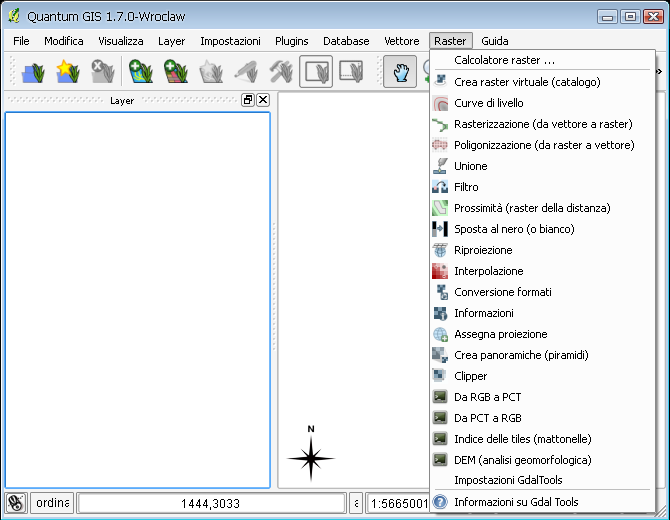
\includegraphics[clip=true, width=12cm]{plugins_gdaltools_images/raster_menu}
\end{figure}

\subsection{Esempi}\label{gdal_examples}
Seguono alcuni esempi di utilizzo degli strumenti GDAL.
\subsubsection{Ottenere informazioni su un raster}

Figura \ref{gdalinfo}.

\begin{figure}
   \centering
   \caption{La finestra di dialogo \emph{Informazioni} \nixcaption}\label{gdalinfo}
   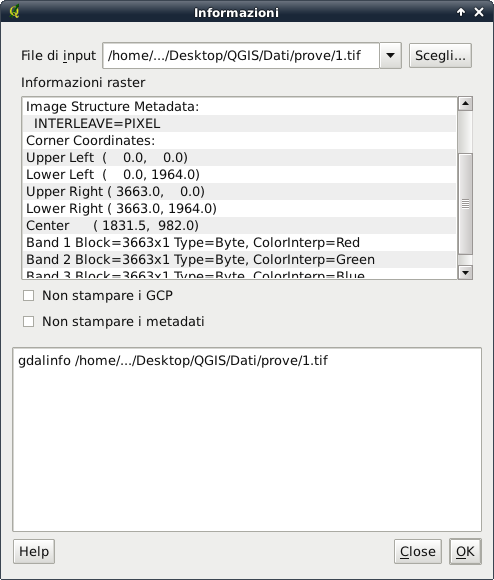
\includegraphics[clip=true, width=10cm]{plugins_gdaltools_images/gdalinfo}
\end{figure}

\subsubsection{Creare curve di livello}
Esempio di creazione di curve di livello da un DEM (Figure \ref{gdal_contour} e \ref{gdal_contour1}).
\begin{figure}
   \centering
   \caption{La finestra di dialogo \emph{Curve di livello} \nixcaption}\label{gdal_contour}
   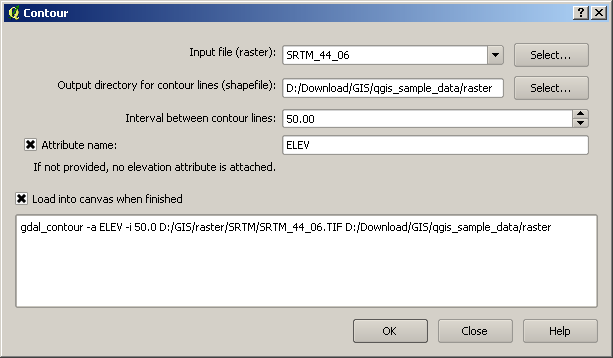
\includegraphics[clip=true, width=12cm]{plugins_gdaltools_images/gdal_contour}
\end{figure}

\begin{figure}
   \centering
   \caption{Layer di curve di livello derivate \nixcaption}\label{gdal_contour1}
   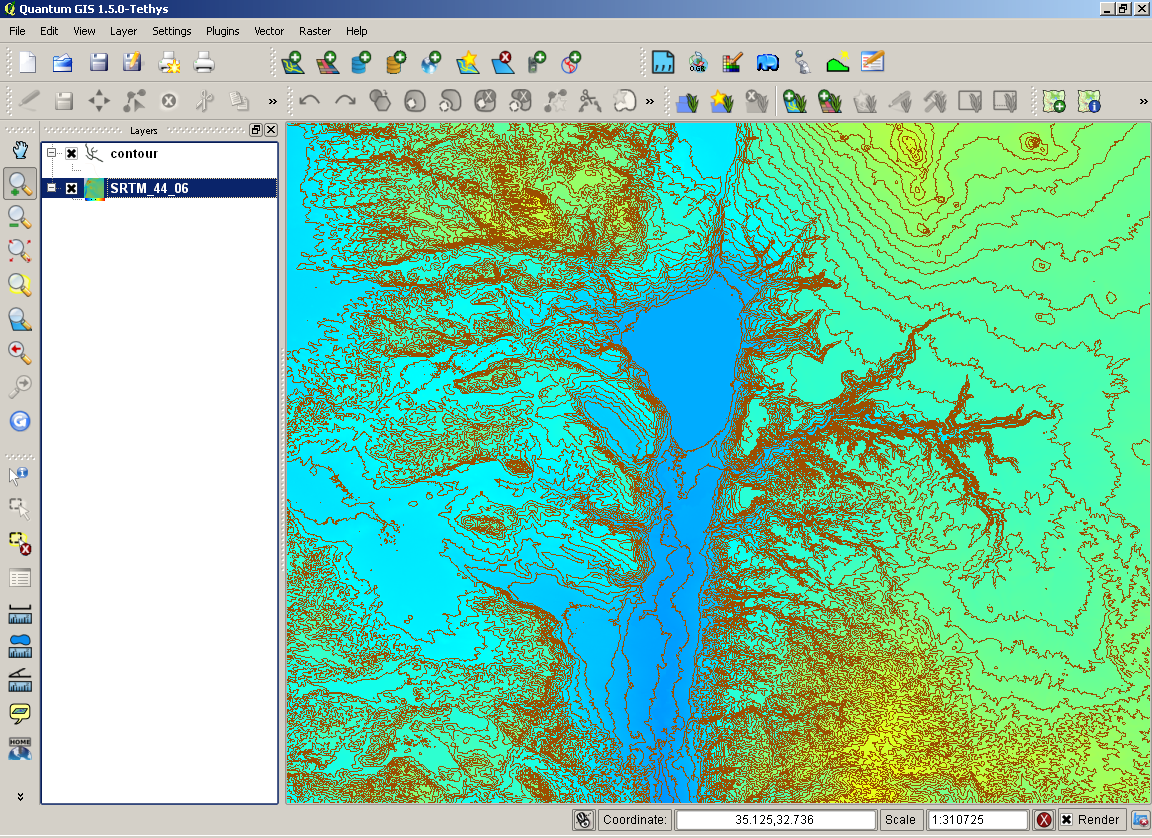
\includegraphics[clip=true, width=12cm]{plugins_gdaltools_images/qgis_contours}
\end{figure}

\subsubsection{Riproiettare un raster}
Esempio per riproiettare un'immagine di una copertura del suolo dalla proiezione 
Albers Equal Area al sistema WGS84 (EPSG:4326) (Figura \ref{gdalwarp}).
\begin{figure}
   \centering
   \caption{La finestra di dialogo \emph{Riproiezione} \nixcaption}\label{gdalwarp}
   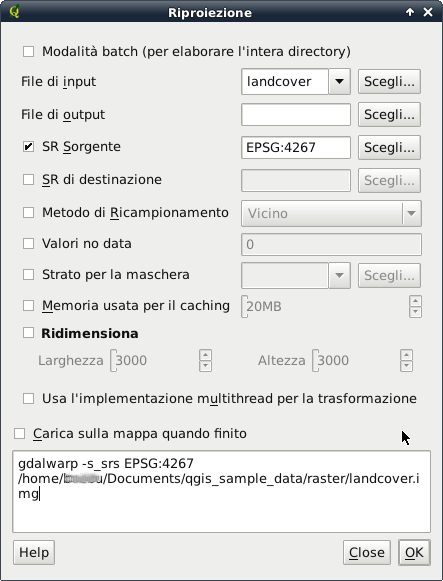
\includegraphics[clip=true, width=12cm]{plugins_gdaltools_images/gdalwarp}
\end{figure}

\FloatBarrier
